\chapter{Il caso di studio} \label{chap:caso_studio}
\section{I social di Meta}
Per il progetto sono stati individuati come obiettivi i due principali social network della societ\`a Meta Platforms Inc.\footnote{\url{https://about.meta.com}}, ovvero Facebook ed Instagram. 
Le due piattaforme sono state selezionate principalmente per il vasto pubblico attivo e conseguentemente per la quantit\`a di informazioni online.
\subsection{Facebook}
Facebook, nato nel 2004, conta ad oggi secondo i dati ufficiali rilasciati dalla societ\`a, 2.93 miliardi di utenti attivi  \footnote{\url{https://investor.fb.com/investor-news/press-release-details/2022/Meta-Reports-Third-Quarter-2022-Results/default.aspx}}. Il social permette di condividere informazioni testuali e multimediali sia pubblicamente che privatamente, attraverso singole pagine personali, pagine pubbliche e gruppi. 
La funzionalit\`a denominata come ``amicizia'' consente la creazione di una rete sociale per ogni singolo utente. 
Le foto, i video, i post, le storie, le reazioni, i commenti, la condivisione di contenuti in diretta, la presenza di un market ed i messaggi istantanei sono i principali punti di forza della piattaforma.
L'imponente diffusione di questo social ha implicato l'impiego dello stesso anche come strumento informativo ufficiale da parte di organi statali, di stampa e di informazione pubblica.
L'aggiornamento costante del servizio aggiunge continuamente nuove funzionalit\`a che vanno ad ampliare la quantit\`a di informazioni pubblicate.

\subsection{Instagram}
Instagram, pubblicata nel 2010, raggiunge ad oggi quasi lo stesso numero di utenti attivi di Facebook. I punti di forza di questo social, nato inizialmente per condividere solamente foto, riuniscono varie possibilit\`a di pubblicazione di informazioni online. Oltre alle semplici foto, possono essere pubblicati altre tipologie di contenuti multimediali come video e musica. La piattaforma consente la pubblicazione dei media sotto forma di post, permettendo agli utenti di cliccare ``mi piace'' e scrivere commenti. Inoltre il singolo utilizzatore pu\`o generare la sua rete sociale tramite il ``follow'' lett. ``seguire'' ed attraversp l'utilizzo il sistema di messaggistica istantanea e la condivisione di storie e post.
I profili degli utenti possono essere impostati come pubblici o privati, questi ultimi necessitano l'autorizzazione del proprietario per essere consultati.
Anche nel caso di Instagram, l'aggiornamento \`e costante in quanto vengono rilasciate costantemente nuove funzionalit\`a a favore degli utenti.


\subsection{Termini e condizioni}
Le piattaforme sopra introdotte individuano termini e condizioni d'utilizzo simili. Nel particolare, in riferimento alla finalit\`a del progetto sviluppato, viene esplicitamente vietato qualsiasi comportamento riconducibile ad azioni di web scraping o pi\`u in generale di collezione dei dati in maniera automatica.\cite{doi:10.1177/2056305120940703}
Come riportato dal file ``robots.txt''\footnote{\url{https://instagram.com/robots.txt}} di Facebook:
\begin{center}
    \textit{``Notice: Collection of data on Facebook through automated means is prohibited unless you have express written permission from Facebook and may only be conducted for the limited purpose contained in said permission. See: \url{http://www.facebook.com/apps/site_scraping_tos_terms.php}''}
\end{center}
Meta contrasta la External Data Misuse (EDM)\footnote{Uso improprio ed esterno dei dati.} promuovendo nuove tecniche contro lo scraping dei dati.
Un deterrente attuato dalla societ\`a \`e anche la promozione di azioni legali contro attivit\`a non consentite dai termini di servizio. Pubblicando notizie ed aggiornamenti su come viene contrastata la collezione automatica di dati si punta a dissuadere un eventuale soggetto interessato all'attivit\`a.
%%%%%%%%%%%%%%%%%%%%%%%%%%%%%%%%%%%%%%%%%%%%%%%%%%%%%%%%continuare


\section{Strumenti Open Source per lo scraping}
Il funzionamento dei singoli connettori di scraping si basa su due tool open source individuati come migliori per lo scopo designato. In particolare, per i due social network oggetto di studio, Facebook e Instagram, si \`e fatto uso rispettivamente di ``facebook-scraper''\footnote{\url{https://pypi.org/project/facebook-scraper/}} e ``instaloader''\footnote{\url{https://instaloader.github.io/}}.

L'individuazione e lo studio di questi strumenti, si \`e basato su un attento confronto delle loro caratteristiche tecniche e di funzionamento.
I due tool utilizzati non impiegano le API ufficiali rilasciate dai rispettivi social. Ci\`o avviene a causa della forte limitazione all'estrazione dati che viene imposta, nel caso specifico da Facebook e Instagram. 

Questa limitazione rende necessario ricorrere a soluzioni che contrastano le linee guida definite dai fornitori dei servizi social, adottando tecniche in grado di eludere i controlli messi in campo e giungere all'obiettivo del progetto garantendo efficienza.

Le piattaforme social vengono continuamente sottoposte a nuovi sviluppi ed aggiornamenti, causando ovvi problemi all'operativit\`a degli strumenti scelti. Ne consegue un continuo aggiornamento dei tool ed una attenta ricerca per la  gestione tecnica del loro funzionamento.

\section{Soluzioni implementative per Facebook}
\subsection{Estrazione e formato dei dati}
Il connettore di Facebook basa il suo funzionamento sul progetto ``facebook-scraper''.
L'acquisizione e la gestione dei dati estratti da questo social network, sono state effettuate con l'obiettivo di essere rese fruibili da parte di sistemi di analisi dati (Big Data Analytics).
Il tool opera direttamente effettuando richieste GET sulle diverse estensioni dei link, a partire da un target\footnote{Si fa riferimento all'obiettivo dell'attivit\`a di scraping.} dato in input.
Nel caso specifico, il route\footnote{Si fa riferimento al percorso definito dal link relativo.} definito dall'API genera l'input per le singole funzioni dello scraper, avviando il processo di identificazione del target e conseguente iterazione sulla gerarchia di link collegati ad esso, ricavando i dati richiesti.
Sono state definite in totale tre route o ``cammini'' per le API, rispettivamente per lo scraping di profili, pagine e gruppi.

Un esempio di route per l'estrazione di tutti i dati di un profilo \`e:
\begin{center}
    localhost:5000/profile/{username}/posts
\end{center}
I dettagli relativi alle singole funzioni sviluppate sono:
\begin{itemize}
    \item \textbf{Profili}: in ``profile.py'' vengono descritte tutte le funzioni per lo scraping di profili pubblici e privati. In particolare si ha la possibilit\`a di scaricare le informazioni generali di un profilo ed anche tutti i post, le foto ed i video, con relativi commenti e reazioni. 
    La funzione ``get\_posts`` di facebook-scraper restituisce un JSON contenente una moltitudine di informazioni da processare. Di conseguenza sono state sviluppate funzioni in grado di elaborare il file JSON ed estrarre ci\`o di interesse.
    Per le foto, osservato che Facebook prevede la presenza di foto in bassa qualit\`a (identificate come anteprime) e foto in alta qualit\`a (identificate come foto dei post) si \`e provveduto a differenziare il download di questi media in funzioni differenti.
    Si riporta in Appendice al paragrafo \ref{scraping_funzioni} il codice per il download dei post e dei media da un profilo.
    \item \textbf{Pagine}: in ``pages.py'' vengono descritte le funzioni per lo scraping di pagine. Come descritto per i profili, anche in questo caso si ha la possibilit\`a sia di estrarre le informazioni generali di una pagine, che i relativi post con media, commenti e reazioni.
    \item \textbf{Gruppi}: in ``groups.py'' sono definite le funzioni per lo scraping di gruppi pubblici e privati. Per i gruppi pubblici valgono le stesse modalit\`a descritte per profili e pagine, mentre per i gruppi i privati lo scraping \`e limitato solo all'estrazioni di informazioni generali e delle indicazioni sugli amministratori. Lo scraping completo di un gruppo privato pu\`o essere effettuato solamente se l'account (ed i relativi cookies) utilizzato per lo scraping risulta appartente al gruppo.
\end{itemize}
Facebook-scraper \`e stato selezionato come migliore servizio da integrare nel funzionamento del connettore di dati dal social Facebook. Il confronto con gli altri tool validi individuati \`e riportato in Tabella \ref{tabella_fb}.

I dati raccolti attraverso l'integrazione di questo tool sono stati sottoposti ad una precisa organizzazione come descritto nel paragrafo \ref{formato dati}.
L'insieme delle qualit\`a descritte in Tabella \ref{tabella_fb} fanno si che facebook-scraper garantisca un'operativit\`a continua nell'estrazione delle informazioni.
In particolare la possibilit\`a di gestione del tempo nelle richieste effettuate consente di simulare la normale attivit\`a di interazione umana con il servizio web, evitando il riconoscimento di automazione con conseguente ban.
Gli ulteriori accorgimenti relativi alle tecniche di elusione dei controlli sono descritti al Paragrafo \ref{contrasto_scraping}.

%\newpage
\begin{table}[!htb]
\centering
\caption{Confronto Tool per Scraping di Facebook.}
\label{tabella_fb}
\begin{tabular}{|p{4,5cm}|p{4,5cm}|p{4,5cm}|}
\hline
\textbf{FACEBOOK-SCRAPER} & \textbf{FACEBOOK-POST-SCRAPER-SELENIUM} & \textbf{FACEBOOK-SCRAPER-SELENIUM} \\\hline
 No API         &  No API                &   No API                        \\\hline
Login non obbligatorio &   Login obbligatorio & Login obbligatorio  \\\hline
Mantenimento di sessione di login & - & - \\\hline
Gestione dei cookies sia in formato NETSCAPE che in formato JSON & - & - \\\hline
Download anonimo completo di profili pubblici e privati & Download anonimo dei soli post di profili pubblici, privati & Download anonimo del solo testo dei post di profili pubblici e privati\\\hline
Download di hashtag, commenti, tag geografici e descrizioni per ogni post & Download di commenti per ogni post (con foto e link) & - \\\hline
Download di tutte le reazioni per ogni post & Download di solo tre reazioni per post & -\\\hline
Download anonimo completo di pagine & Download anonimo dei post delle pagine & Download anonimo dei post delle pagine \\\hline
Download anonimo di gruppi pubblici e privati & - & Download dei post dei gruppi pubblici e privati \\\hline
Download di file JSON & Download di file JSON & Download di file CSV\\\hline
I media vengono estratti tramite metodo GET & I media vengono estratti tramite metodo GET & -\\\hline
\end{tabular}
\end{table}
\begin{table}[!htb]
\begin{tabular}{|p{4,5cm}|p{4,5cm}|p{4,5cm}|}
\hline
Personalizzazione di filtri di ricerca & - & -\\\hline
- & Utilizzo di ``Selenium'' & Utilizzo di ``Selenium'' \\\hline
Download in elenco degli amici & - & - \\\hline
Il download di profili privati avviene solo se l’account usato fa parte della lista degli amici dall’account target & Il download di profili privati avviene solo se l’account usato fa parte della lista degli amici dall’account target & Il download di profili privati avviene solo se l’account usato fa parte della lista degli amici dall’account target \\\hline
Orientato al solo scraping di profili di terzi & Orientato al solo scraping di profili di terzi & Orientato al solo scraping di profili di terzi \\\hline
\end{tabular}
\end{table}
\newpage


\subsection{Risoluzione del contrasto}
Durante il funzionamento del tool, si incorre facilmente in errori dovuti alle soluzioni anti-scraping. In particolare si ricevono i seguenti codici di stato\footnote{Codici di stato HTTP, indicano l'esito di una comunicazione HTTP} e comunicazioni:
\begin{itemize}
    \item \textbf{429 Too Many Requests}: il codice di stato 409 viene presentato quanto viene superato il limite di richieste da parte di un indirizzo IP in un determinato arco temporale. Una volta presente questo codice, sar\`a necessario riavviare il processo di scraping.
    \item \textbf{Temporary Ban}: errore presentato quando \`e stata individuata un'attivit\`a sospetta da parte di un account. Da test effettuati, il ban temporaneo di un profilo dura 24/48 ore, successivamente torna ad essere operativo.
    \item \textbf{Account disabled}: qualora un account sottoposto a un ban temporaneo continui ad effettuare richieste, viene presentato l'errore e la comunicazione di ban permanente a causa dell'attivit\`a non consentita. L'account non risulter\`a essere pi\`u recuperabile.
    \item \textbf{Unusual Activity}: avviso di attivit\`a sospetta proveniente da un account. Viene bloccata l'attivit\`a in corso senza ulteriori ``provvedimenti''. Nel caso in cui lo stesso account, con lo stesso IP, continui operazioni di tipo massivo, si incorrer\`a in modo certo a un ban temporaneo.
\end{itemize}
Per limitare la comparsa degli errori sopra riportati \`e stato sviluppato un sistema di rotazione dei cookies, come presentato al paragrafo \ref{cookie rotation}.

I cookie all'interno del progetto sono stati gestiti ed utilizzati per il login degli account utilizzati per lo scraping. La gestione si \`e basata sulla estrazione e memorizzazione dei valori necessari per il funzionamento dei tool scelti.

Per estrarre i cookie relativi alla sessione dei singoli account si \`e fatto uso di Selenium, grazie al quale, automatizzando le operazioni su browser Chromium in modalit\`a headless, si sono potuti estrarre i valori dei cookie di interesse per il login.

Si riporta il codice relativo all'implementazione di Selenium ed un esempio dei valori dei cookie estratti in Appendice \ref{cookie_code}.

La funzione ``cookie\_rotation'' ha consentito il mantenimento di una continuit\`a operativa del tool, grazie all'elusione dei controlli.
Si riporta il codice della funzione:
\inputminted[bgcolor=bg]{python}{codice/cookie_rotation_fb.txt}

Oltre alla soluzioni adottata sui cookie, si \`e prevista per ogni azione di download con richieste dirette al server target, l'aggiunta di tempi d'attesa nell'ordine dei secondi. Rallentando l'attivit\`a si \`e aumentata la resistenza del tool contro eventuali azioni di ban, immedesimando l'utilizzo del social da parte di un umano, inteso come utente reale e non bot.
\begin{center}
\begin{minted}[bgcolor=bg]{python}
time.sleep(15)
\end{minted}
\end{center}
La funzione ``time.sleep'' in Python, sospende l'esecuzione di un determinato processo sulla base del numero di secondi inseriti in input.

Tutte le funzioni elencate necessitano di login con account validi. La gestione degli account avviene attraverso la memorizzazione delle credenziali in file JSON, dal quale vengono estratte per avviare i processi di login.
\subsection{Aggiornamenti}
A causa dell'attivo e consistente contrasto ed all'aggiornamento tecnico delle infrastutture dei social, durante lo sviluppo si sono presentate diverse problematiche relative al corretto funzionamento dello scraping.
Ogni questione \`e stata prontamente risolta grazie al rilascio di nuove versioni del tool.
La cronistoria dei rilasci \`e presente nello schema riportato al paragrafo \ref{confronti_software}.

\section{Soluzioni implementative per Instagram}
\subsection{Estrazione e formato dei dati}
Il connettore di Instagram basa il suo funzionamento sul progetto ``instaloader''.
Instaloader consente il download di profili completi di media (foto e video) e metadati\footnote{Serie di informazioni aggiuntive sui dati.} per ogni post.
L'acquisizione e la gestione dei dati estratti da questo social network, sono state effettuate con l'obiettivo di essere rese fruibili da parte di sistemi di analisi dati (Big Data Analytics). 

Instaloader \`e stato selezionato dopo la comparazione del suo funzionamento con altri tool open source individuati. Il confronto \`e riportato in Tabella \ref{tabella_insta}.
L'attivit\`a effettuata con instaloader ha subito una organizzazione e gestione simile a quella di facebook-scraper.
Le principali differenze, riguardanti l'approccio di funzionamento del tool, sono state uniformate con particolare attenzione alla gestione dei dati in output.

Lo sviluppo dell'API prevede la presenza di route, le quali generano l'input per le singole funzioni dello scraper, avviando l'iterazione sulla gerarchia di link collegati al target, ricavando i dati richiesti.
Un esempio di route per l'estrazione dei post con il connettore di Instagram \`e:
\begin{center}
    \url{localhost:5000/<username>}
\end{center}

Anche nel caso di Instagram, le attivit\`a messe in campo per l'elusione dei controlli anti-scraping sono descritte al Paragrafo \ref{contrasto_scraping}.

Le principali funzioni sviluppate ed impiegate per lo scraping di questo social sono:
\begin{itemize}
    \item \textbf{Post, foto e video}: la funzione ``profile\_dl'' consente di estrarre tutti i post di un profilo pubblico senza effettuare il login e tutti i post di un profilo privato se si effettua il login e se l'account in uso fa parte dei follower approvati dal target. \`E possibile anche effettuare il download dei post in cui l'obiettivo \`e stato taggato. La funzione prevede un controllo della frequenza delle richieste, limitando il numero delle stesse ed aggiungendo ritardo nell'ordine dei secondi. Insieme ai media relativi a tutti i post viene memorizzata anche la foto profilo dell'account.
    Per ogni post estratto, viene memorizzato anche un file JSON contenente informazioni aggiuntive come i commenti, il numero di mi piace, l'eventuale posizione GPS, la data e l'ora di pubblicazione, le informazioni del profilo, eventuale connessione del profilo con un account Facebook ed altri metadati. 
    \item \textbf{Storie}: la funzione ``stories\_dl'' consente di estrarre tutte le storie valide\footnote{Per validit\`a di una storia si fa riferimento, secondo le policy di Instagram, al contenuto pubblicato entro le 24 ore dalla visione.} pubblicate da un utente. La funzione necessita di login al social e prevede il controllo della frequenza. 
    \item \textbf{Followers e seguiti}: le funzioni ``followers\_dl'' e ``followee\_dl'' prevedono la possibilit\`a di restituire in output elenchi in JSON dei follower e dei seguiti dell'account target. Necessitano di login e sono molto vulnerabili alle azioni di contrasto. La loro vulnerabilit\`a nasce dal numero di elementi da estrarre. Nella maggioranza dei casi, il numero di follower o di seguiti \`e maggiore rispetto al numero di post pubblicati ed appartenente all'ordine delle centinaia o migliaia. Ne consegue che il numero di richieste segue il numero di elementi, esponendo l'azione al controllo.
    \item \textbf{Geolocalizzazione}: la funzione ``location\_dl'' consente, a partire dall'input di un luogo, di effettuare l'estrazione di tutti i post geolocalizzati in quel punto. Ne consegue che questa funzione rappresenta un'estensione rispetto al normale download dei post da un profilo, in quanto estende la possibilit\`a di ricerca sulla base della posizione.
\end{itemize}
Il tool offre la possibilit\`a di analizzare il comportamento storico di un utente, confrontando i dati gi\`a scaricati e memorizzati rispetto ad una nuova azione di scraping. Ci\`o oltre ad evitare ridondanza, consente anche di ottimizzare le richieste al server, riducendone il numero.

Anche in questo caso, tutte le funzioni elencate che necessitano di login con account validi, gestiscono le credenziali attraverso file JSON, dal quale vengono estratte per avviare i processi.

Tutti i media vengono memorizzati nella qualit\`a massima, ovvero la stessa presente alla normale fruizione dei dati dal social. 
Si riportano in Appendice al Paragrafo \ref{scraping_funzioni_insta} le funzioni di scraping adottate per lo sviluppo del connettore.
%\newpage
\clearpage
\begin{table}[!htb]
\centering
\caption{Confronto Tool per Scraping di Instagram.}
\label{tabella_insta}
\begin{tabular}{|p{4,5cm}|p{4,5cm}|p{4,5cm}|}
\hline
\textbf{INSTALOADER} & \textbf{INSTAGRAPI} & \textbf{INSTAGRAM-SCRAPER-2021-SELENIUM} \\\hline
No API & Basato su API ufficiale di Instagram & No API \\\hline
Login obbligatorio per alcune azioni & Login obbligatorio & Login obbligatorio\\\hline
Supporto autenticazione a due fattori & Supporto autenticazione a due fattori & Supporto autenticazione a due fattori \\\hline
Download anonimo di profili pubblici e privati & Download anonimo di profili pubblici, privati & Download anonimo di profili pubblici, privati \\\hline
Il download di profili privati avviene solo se l’account usato fa parte della lista dei follower dell’account target & Il download di profili privati avviene solo se l’account usato fa parte della lista dei follower dell’account target & Il download di profili privati avviene solo se l’account usato fa parte della lista dei follower dell’account target \\\hline
Download di storie, mi piace, commenti e tag geografici & Download di storie, mi piace, commenti e tag geografici & -\\\hline
Download diretto di foto e video & - & - \\\hline
Download dei file in JPG, MP4 e JSON & Download di file JSON & Download di file JSON \\\hline
- & - & Utilizzo di Selenium \\\hline
Rilevazione di cambio di username & - & -\\\hline
Rilevazione dei post eliminati & - & - \\\hline
\end{tabular}
\end{table}
\clearpage
\begin{table}[!htb]
\begin{tabular}{|p{4,5cm}|p{4,5cm}|p{4,5cm}|}
\hline
Download di metadati aggiuntivi & - & -\\\hline
Personalizzazione di filtri di ricerca & - & - \\\hline
Mantenimento di sessione di login & - & - \\\hline
Permette il download di post appartenenti ad uno specifico periodo temporale & - & -\\\hline
Rilevazione automatica e continuazione di download interrotti & - & - \\\hline
- & Challenge resolver (per verification code login su email e sms) & - \\\hline
Presenza di buon supporto da parte della community & - & - \\\hline
\end{tabular}

\end{table}


\subsection{Risoluzione del contrasto} \label{risoluzione_insta}
Come per il tool di Facebook, anche per lo scraping di Instagram, si presentano errori dovuti alle soluzioni anti-scraping:
\begin{itemize}
      \item \textbf{429 Too Many Requests}: il codice di stato 429 viene presentato quanto viene superato il limite di richieste da parte di un indirizzo IP in un determinato arco temporale. Una volta presente questo codice, sar\`a necessario riavviare il processo di scraping.
      \item \textbf{401 Unauthorized}: il codice 401 viene presentato quando si tenta di effettuare il download di dati da profili privati o senza aver effettuato il login al servizio.
      \item \textbf{Ban}: diversamente da quanto accade con Facebook in cui \`e presente anche un soft-ban, per Instagram il ban di un profilo risulta essere definitivo in caso di azioni non consentite. Ci\`o avviene con pi\`u frequenza quando ad le azioni non riconosciute sono effettuate da un account appena creato. Lo studio e lo sviluppo del connettore ha evidenziato come Instagram attui una politica di controllo nei confronti di account appena creati, attenzionando e limitando il numero di operazioni consentite.
      \item \textbf{Riconoscimento ``umano'' anti-bot}: una volta che un account \`e stato segnalato a causa di azioni sospette, viene richiesta l'identificazione personale del soggetto per eliminare eventuali bot. Nel caso in cui ci\`o non avvenisse, il profilo verr\`a sottoposto a ban permanente. Si riporta schermata di richiesta fotografia ``selfie'' con specifiche azioni da effettuare per il riconoscimento dell'utente in qualit\`a di persona fisica proprietaria dell'account.

\end{itemize}
  \begin{figure}[!htb]
          \centering
          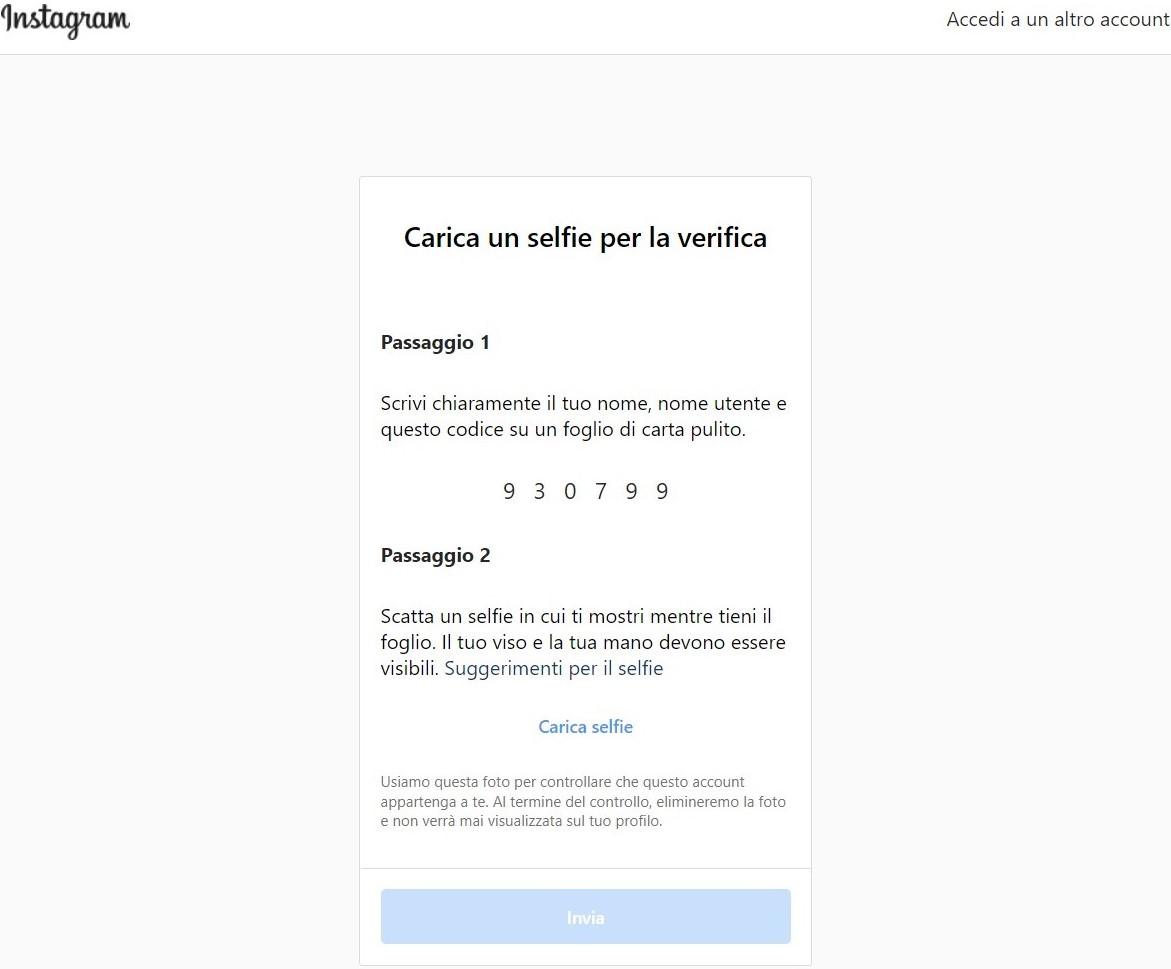
\includegraphics[width=400pt]{immagini/login_selfie.jpg}
    \end{figure}
\newpage

Lo studio e lo sviluppo di tecniche di elusione dei controlli e del contrasto sopra descritto si \`e attuato adottando le stesse idee implementative del connettore di Facebook.

In questo caso, come fatto per la funzione ``cookie\_rotation``, osservando la diversa gestione dei cookie da parte del tool per il connettore di Instagram, si \`e sviluppata una funzione di ``account\_rotation'' di cui si riporta il codice.

\inputminted[bgcolor=bg]{python}{codice/account_rotation_insta.txt}

\subsection{Aggiornamenti}
Come descritto per il connettore di Facebook, le problematiche di sviluppo del connettore e di impiego del tool instaloader sono state causate, oltre che dalle soluzioni anti-scraping, dagli aggiornamenti della piattaforma.
Le maggiori difficolt\`a affrontate nello sviluppo hanno riguardato la gestione del login al servizio, continuamente aggiornata da Instagram sia in termini di funzionalit\`a che in termini di sicurezza.

Al Paragrafo \ref{confronti_software} viene presentata la cronistoria degli aggiornamenti del tool su cui si basa il connettore.
\section{Tecnologie utilizzate} \label{tecnologie_utilizzate}
Le soluzioni tecniche adottate per lo sviluppo di questo progetto sono state basate sul concetto di portabilit\`a e operativit\`a continua del servizio di raccolta dati. 

Il linguaggio scelto per lo sviluppo del progetto \`e stato Python\footnote{\url{https://www.python.org/}}, il quale grazie alla vasta offerta di librerie e strumenti dedicati, \`e risultato essere idoneo ad applicazioni di Web Scraping e di analisi ed elaborazione dati.
Inoltre Python si presenta come uno strumento vantaggioso per lo sviluppo di API\footnote{Application Programming Interface.}, fondamentali per permettere il riuso del codice e garantire un utilizzo e un'inclusione delle funzionalit\`a da parte di altri sviluppatori. 

Le scelte tecnologiche adottate sono state definite tramite l'impiego di strumenti Open Source, di formati dati universali e leggibili e di paradigmi architetturali per lo sviluppo web.

Lo sviluppo e l'impiego di software container, ha permesso di massimizzare la portabilit\`a del servizio, garantendo uniformit\`a e produttivit\`a.

L'individuazione di tool open source si \`e basata su uno studio e confronto delle carattistiche, ponendo attenzione anche all'attivit\`a e al seguito delle community di sviluppatori, in modo tale da garantire continuit\`a e costanza nell'aggiornamento dei servizi.

\subsection{Formato dei dati}\label{formato dati}

Lo standard individuato per la gestione dei dati estratti \`e il formato JSON.

JSON \`e un formato di testo per la serializzazione di dati strutturati basato sul linguaggio di programmazione JavaScript, dal quale per\`o non dipende.
JSON rappresenta quattro tipi di dato fondamentali (stringhe, numeri, valori booleani e nulli) e due tipi strutturati (oggetti e vettori).\cite{bray2014javascript}
Grazie alla sua chiara sintassi, rappresenta uno standard interpretabile facilmente sia da persone che da macchine garantendo portabilit\`a e interoperabilit\`a multipiattaforma, fondamentale per l'impiego delle API sviluppate in questo progetto.

L'alta leggibilit\`a del formato JSON ha permesso una manipolazione dei file di output, garantendo soluzioni tecniche idonee per la successiva estrazione dei dati.

La successiva soluzione per il salvataggio dei dati richiesti si basa su formati standard di file multimediali come MP4 e JPG. Essendo lo scraping massivo di dati e la conseguente ingestione in sistemi di analisi dati l'obiettivo finale del progetto, si \`e reso necessario comprimere tutti i dati raccolti in formato ZIP.

Il formato ZIP \cite{zip} è un formato di compressione dati senza perdita di informazioni in grado di ridurre lo spazio occupato dai file.
L'utilit\`a della compressione dei file si rende fondamentale nel processo di ingestione dei dati in sistemi di Big Data Analytics.



\subsection{API}

Il progetto si \`e basato sullo sviluppo di API RESTful utilizzando il servizio Flask\footnote{\url{https://flask.palletsprojects.com/en/2.2.x}}.

Flask \`e un framework per applicazioni web, caratterizzato dalla sua leggerezza ed ampia compatibilit\`a. Offre scalabilit\`a e gestione di progetti complessi, non richiedendo specifici strumenti o scelte progettuali; in questo modo vengono favorite le opzioni implementative delineate dello sviluppatore.
Le funzionalit\`a di Flask impiegano due dipendenze: Werkzeug\footnote{\url{https://werkzeug.palletsprojects.com/en/2.2.x}} e Jinja2\footnote{\url{https://jinja.palletsprojects.com/en/3.1.x}}.
Werkzeug gestisce le attivit\`a di routing, debugging ed il protocollo di trasmissione WSGI\footnote{Web Server Gateway Interface.}, mentre Jinja2 gestisce i template per le API.
Lo sviluppo di API REST tramite Flask consente di instanziare le singole applicazioni, associando singoli route (percorsi) alle varie funzioni, sotto forma di URL.
La risposta alle varie richieste, fornita dal server, fornisce in aggiunta un HTTP Response (codice) che, a seconda del caso, individua un successo o un errore di client o server.\cite{grinberg2018flask}

Si riporta un estratto di codice del connettore di Facebook inerente all'utilizzo di Flask in Appendice \ref{flask_code}.



\subsection{Docker}
Entrambi i connettori sono stati posti in container utilizzando Docker. Come introdotto al Paragrafo \ref{software_container}, per la creazione dell'immagine occore generare il rispettivo Dockerfile. In appendice si riporta a titolo d'esempio il Dockerfile per il connettore di Facebook (Paragrafo \ref{dockerfile}).





\subsection{Strumenti di automazione}
L'automazione del software viene impiegata nell'ambito del testing dei servizi e dell'interazione automatica con elementi dell'interfaccia utente. In questo progetto, \`e stato individuato Selenium come strumento open source in grado di effettuare operazioni automatiche sui browser.

Selenium\footnote{\url{https://www.selenium.dev/}} consente di automatizzare delle operazioni su browser web, consentendo anche l'estrazione di informazioni visive.\cite{gundecha2015selenium}
L'impiego di Selenium nel progetto \`e consistito nell'accesso automatico ai siti web di interesse e nell'estrazione dei valori relativi ai cookies persistenti (descritti al paragrafo \ref{cookieitem}). 

Il funzionamento di Selenium \`e basato sull'interpretazione e la creazione di richieste HTTP per ogni comando scritto dallo sviluppatore. Ogni comando viene successivamente inviato al driver del browser individuato come ambiente di testing e di lavoro. Sono supportati i maggiori browser quali Chrome/Chromium, Firefox, Edge, Explorer e Safari. 
Per le scelte progettuali, osservato l'impiego di container basati su Linux, l'automatizzazione \`e stata implementata con driver Chromium\footnote{\url{https://www.chromium.org/chromium-projects/}}.

Grazie alla possibilit\`a di impostare il WebDriver in modalit\`a headless\footnote{Headless Browser, assenza di interfaccia grafica.}, sono stati recuperati automaticamente i dati aggiornati dei singoli account da impiegare, garantendo operativit\`a continua.

